\chapter{Design and implementation}

This chapter will describe details of implementation and design of my test application.
Starts with listings frameworks that were used and describes process of incorporation of the application into that frameworks.
Then few design details concerning the incorporation is described.
After that results of profiling of the application are summarized.
Followed by new design description which was neccessary due to unexpected profiling results.
The rest of chapter will present actual porting process with all its problems and solutions.

\section{Used frameworks}

\par
We decided to take ITK (\url{www.itk.org}) implementation of level set method as a base.
So we have to get familiar with this huge project.
It contains many algorithm implementations as well as necessary infrastructure content such as loading and saving variety of formats.
Base concept of this project is pipeline and filters.
To get some work done pipeline has to be build from filters.
Filter is entity that represent an algorithm.
When pipeline is created the last filter is started.
Starting event then propagate towards the begining of the pipeline where actual computation starts.
Output from one filter is input of the following.
Filters thus create a building blocks for some more complicated method.

\par
After some first test with example implementation we wrote our own testing application (originally with code name 'pok').
It was able load image, run the level set filter and save the results.
Some reasonable parameter values were found with the pok application.
It was controlled via bash scripts that is not much easy nor user friendly.
There was also no way how to visualize the results.
So we decided to use another framework to overcome this problems, the Medv4D project (\url{http://cgg.mff.cuni.cz/trac/medv4d}).

\par
This project that was originally started as software project and is basically framework for creation of medical applications.
Its purpose is to simplify process of GUI creation as well as actual computation model design.
Instead the programmer should focus on actual problem solution.
Basic building block is also a filter.
The filter can be merged into pipeline just like in ITK.
But the Medv4D filters are more low-level and thus faster that ITK ones (speed was another goal of the framework).
The pipeline then offer some implicit locking of dataset parts to allow parallel computation.

\section{Incorporation into Medv4D framework}

\par
The most convenient way how to incorporate ITK pipeline that is to be run on Cell B.E. seemed client/server architecture.
So the part of the application that has to be run on Cell B.E. is server.
While client part loads initial data (and saves the results), visualize the results and act as GUI with controls for parameter tuning.
Whole process can be described this way: client loads the input data sends them to server and waits for the results.
As soon as the results is read it is visualized.
Then the result can be saved or sent to server again for computation with another parameters.
See figure \ref{fg:computationProcess} showing how the application with code name 'RemoteCellLevelSet' works.

\begin{figure}
    \centering
    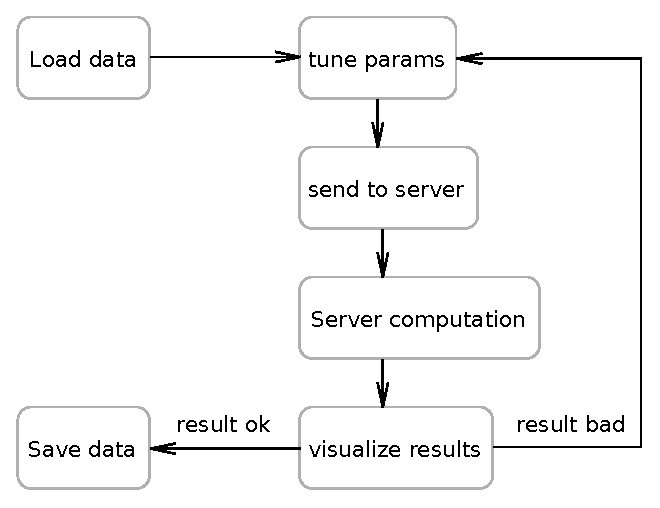
\includegraphics[width=0.7\textwidth]{data/computationProcess}
    \caption[RemoteCellLevelSet application computation process]{Client acts like GUI for the server side that performs actual computation}
    \label{fg:computationProcess}
\end{figure}

\par
There were two main goals which were necessary for incorporation 'pok' into
Medv4D framework:
\begin{enumerate}

  \item{Remote computing infrastructure}
  \par
  Infrastructure for sending commands to server along with data or parameter values as well receiving response messages along with resulting data had to be implemented into Medv4D.
It lead into designing whole new library of Medv4D called remote computing.
On client side it is representing by a remote filter that encapsulate whole infrastructure necessary for sending part of pipeline that the filter represents to server as well as result handling.
Server side had to be designed completely as a whole.

  \item{ITK integration}
  \par
  This is performed by wrapper Medv4D filter that is connected into Medv4D pipeline.
Within this filter are two ITK images that serves as input and output for inner ITK pipeline.
Actual data of this ITK images point to data of containing Medv4D wrapper filter (see figure \ref{fg:ITKWrapping} for details).

\end{enumerate}

\begin{figure}
    \centering
    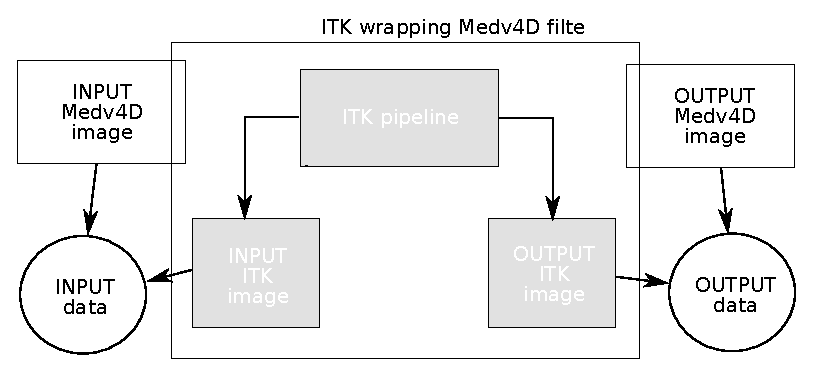
\includegraphics[width=0.9\textwidth]{data/ITKFilter}
    \caption[ITK wrapper Medv4D filter]{Basic elements are the two ITK images whose data are actually Medv4D images' data}
    \label{fg:ITKWrapping}
\end{figure}

\subsection{Client remote computing (RC) part}

As mentioned above base element of client RC part is remote filter.
It implements actual command sending and result receiving functionality.
It is derived from pipeline Medv4D filter so it can be added into pipeline.
This part of pipeline that the remote filter represents thus run on remote server.
Listing of commands that the remote filter issue to the server:
\begin{enumerate}
  \item{CREATE}
  \par
  This command is create request.
It identify the type of the filter that the remote filter represents and that should be instantiated on the server.
Server parses the command message and instantiate appropriate filter along with whole pipeline (remote pipeline).

  \item{DATASET}
  \par
  Tells the server to read actual dataset that the computation will be performed on.
The dataset is parameter of the command.

  \item{EXEC}
\par
  Is request for actual execution of the remote pipeline.
But before that parameter of this command which are filter parameter values should be parsed.
After the parsing and association of filter parameters with actual filter is the remote pipeline executed.
\end{enumerate}

\par
Purpose of the commands is to divide actual execution into stages and thus to define a state of remote execution.
This is because when actual dataset is send to server it would be worthless to send it again when user wants to execute remote pipeline again only with different parameters.
So commands allow this because remote pipeline has state telling 'data already recieved now waiting for EXEC command as many times as wanted without no more input data transmission'.
\par
The Medv4D pipeline filter defines also some stages that the behaviour of remote filter benefits.
That is there are method that is called only when input data changes (PrepareOutputDataset).
This is perfect place to send DATASET command to server.
Because this is called only on input data change thus DATASET command will be issued on input data change as well.
\par
CREATE command is sent in constructor of remote filter thus when pipeline is constructed which is usually at program startup.
And EXEC command is then send within function that is called when pipeline is executed and that should perform actual computation (ProcessImage).
Whole cycle shows figure \ref{fg:RCClientCycle}.

\begin{figure}
    \centering
    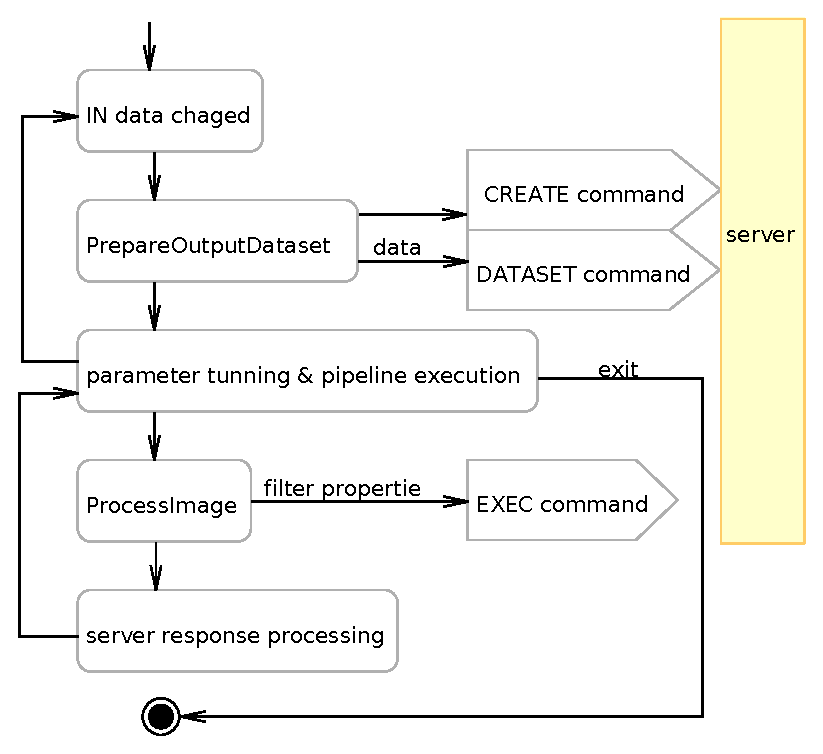
\includegraphics[width=0.8\textwidth]{data/RCClientCycle}
    \caption[Remote Medv4D filter]{Shows three basic states of remote filter and when particular command are sent to server.}
    \label{fg:RCClientCycle}
\end{figure}

Server response can be either OK or FIALED.
In case of OK resulting dataset is received in contrast to FAILED case when no dataset is expected.

\subsection{Server RC part}

Server part is counter part of client one so the design reflects it.
Goal of server is to sit and wait for incoming connection.
One connection means one session of computation.
Currently only one session at a time is held.
In context of a session command from client are parsed and appropriate actions performed (see figure \ref{fg:RCServerCycle}).

\begin{figure}
    \centering
    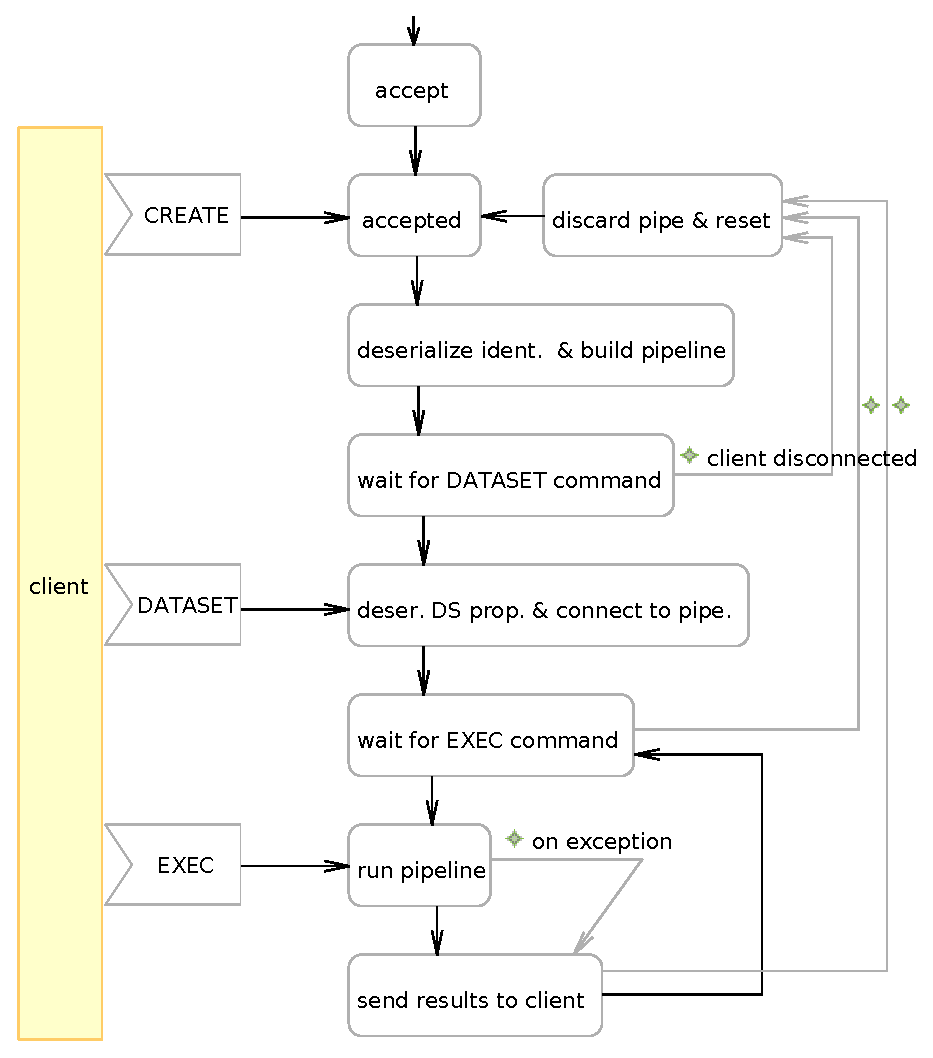
\includegraphics[width=0.9\textwidth]{data/RCServerCycle}
    \caption[MedV4D server cycle]{}
    \label{fg:RCServerCycle}
\end{figure}

Like in every client/server application some kind of stubs are needed.
In context of RemoteCellLevelSet application client/server pair the meaning of the stubs are serialization and de-serialization methods.
Goal of the methods is ensure that data that the client sends will be received in exactly the same order and data types.
Good example is the CREATE request.
In this request identifier of remote filter are send along with template parameters identifiers (because filter classes are templated).
In case of mismatch of that identifiers completely different class would be instantiated.
Hierarchy of virtual methods on dataset classes defines interface for such stubs.
Interface on remote filter properties class hierarchy does the same for remote filter.

Another issue is endianess.
Endianess identifier is sent along with every command. On the other side is made decision if byte swapping should be performed.
This allows to perform byte swapping only when it is really needed.

Currently only remote filter is implemented, the level set segmentation.
But other filters can be easily added by appending one switch branch in remoteFilterFactory.cpp source.
The level set segmentation filter is implemented as successor of ITK filter that contains appropriate ITK pipeline within.
This pipeline is most interresting part related to this work so further content will be about it.

\section{Level set segmentation pipeline}

This pipeline contains three ITK filters.
\begin{enumerate}
  \item{fast marching filter}
  \par
  Is responsible for computation of initial level set.
Parameters of this filter are point $\vec{x}$ in dataset and distance $d$.
Output is then level set that corresponds to ball shaped level set with radius $d$.

  \item{level set segmentation filter (LS Filter)}
  \par
  Performs actual level set segmentation method.
Parameters of this filter are threshold interval (thresholding level set segmentation),  maximal count of algorithm iterations (explained later), curvature and speed scaling (explained above).

  \item{binary thresholding filter}
  \par
  Purpose of this filter is extract resulting object from level set.
It is thresholding that select pixels with values less that zero that corresponds to inner part of the resulting level set.
\end{enumerate}

We have chosen ITK sparse field method implementation to port to Cell B.E.
This implementation uses linked lists to represent the sparse field layers.
Actual algorithm, as described higher (\ref{alg:sparseFileld}), is implemented in several classes.
Due to mapping the algorithm to Cell B.E. radical changes in code was necessary even in ITK code.
We decided to rebuild appropriate part of ITK class hierarchy responsible for the sparse field level set computation (LS hierarchy) to create actual LS Filter.
We borrowed some part of original code and inherited my classes from classes close to finite difference solver (FDS) class, see figure\ref{fg:originalHierarchy}.
In the original LS hierarchy are actually two class hierarchies.
One represents the filter that performs level set algorithm, the filter hierarchy.
The other finite \emph{difference function} that computes the finite differences (the upwind scheme), the function hierarchy.

At the top of the function hierarchy is FiniteDifferenceFunction that computes the 'upwind scheme' with assistance of virtual methods, that are implemented in successors.
Successors are:
\begin{enumerate}
  \item{LevelSetFunction}
  \par
  that provides curvature term computation methods.

\item{SegmentationLevelSetFunction}
\par
provides speed image computation infrastrucutre

\item{ThresholdSegmentationLevelSetFunction}
\par
computes actual speed image
\end{enumerate}

In the filter hierarchy, everything starts with FiniteDifferenceImageFilter that computes main loop of level set calculation (see step 1 in \ref{alg:sparseFileld}).
Virtual methods of its successors are used (just like in function hierarchy) to implement sub steps.
Successor is the SparseFieldLevelSetImageFilter providing implementation of Step 1a through \emph{update calculation} function.
Other steps is performed by \emph{apply update calculation} function.
Next successors, SegmentationLevelSetImageFilter and ThresholdSegmentationLevelSetImageFilter only manage \emph{difference function} in their own manner.
In case ThresholdSegmentationLevelSetImageFilter manages speed function as described in \ref{eq:speedFunction}.
It preallocates another image for pre-calculation of the speed function.
This another image is another notable amount of memory that can not be accepted for my purpose (see \ref{ps3MemoryUsage}).
This pre-calculation was one reason of inheritance from classes close to FDS.
Speed function is calculated every time it is needed without any pre-calculations in my approach.
This approach could be even better for Cell B.E. streaming nature.
The second reason was to simplify the structure of hierarchy and some code clean-up and refactorization.

\begin{figure}
    \centering
    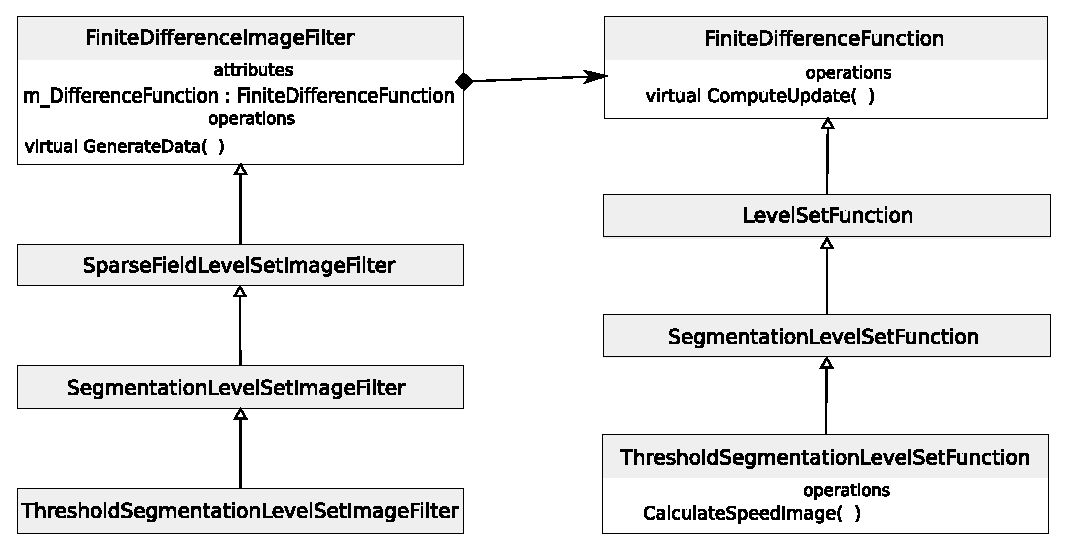
\includegraphics[width=0.9\textwidth]{data/originalHierarchy}
    \caption[Original ITK thresholding level set filter class hierarchy]
{Illustrates the FiniteDifferenceFunction hierarchy and the FiniteDifferenceImageFilter hierarchy and their relationship}
    \label{fg:originalHierarchy}
\end{figure}

Result of this changes is our own filter (ThreshSegLevelSetFilter) that omits all unnecessary part of original LS hierarchy, uses reasonable parts of the original ITK level set segmentation filter and is ready to be ported for Cell B.E. (see figure\ref{fg:resultingFilter}).
In the function hierarchy stayed only the base class that the resulting ThresholdLevelSetFunc class is derived.
This new class does the same job as original LS function hierarchy but in manner closer to streaming architecture (the pre-allocation of the speed image is omited).
The computation of particular up-wind scheme terms was separated into stand alone classes for more code readability and modularity.
The filter hierarchy was shorted and begins already in SparseFieldLevelSetImageFilter.
All the successors in original hierarchy was omited since they did anything reasonable.
Some function implementation from the SparseFieldLevelSetImageFilter was borrowed into the new ThreshSegLevelSetFilter to be tuned for Cell B.E.

\begin{figure}
    \centering
    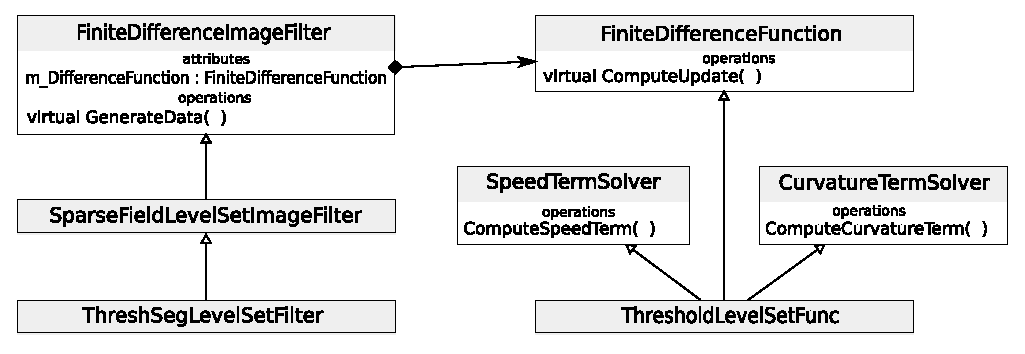
\includegraphics[width=0.9\textwidth]{data/resultingFilter}
    \caption[Resulting level set filter ready to be ported to Cell B.E.]
    {
Show result of original LS hierarchy rebuilding.
Some unnecessary parts was omited to clean-up the code and to change behaviour towards streaming architecture as well as term computation was separated into supporting classes for modularity
    }
    \label{fg:resultingFilter}
\end{figure}

\section{Profiling}

Server application with the thresholding level set filter within was build and then profiled. As the first step of the porting process.

\begin{table}
\centering
\begin{tabular}{|c|c|c|c|}
\hline
\multicolumn{4}{|c|}{Profiling results}\\
\hline
function name&subroutine&time spend&percent\\&&in calculations&\%\\&&(in seconds)&\\
\hline
\hline
ApplyUpdate()&&20.15&75.21\\
\hline
&PropagateAllLayerValues()&16.64&62.11\\
\hline
&UpdateActiveLayerValues()&2.27&8.47\\
\hline
CalculateChange()&&6.11&22.8\\
\hline
&ComputeUpdate()&3.97&14.82\\
\hline
TOTAL&&26.79&100\\
\hline
\end{tabular}
\par
\caption[Profiling results]
{
  Results of profiling showed that ComputeUpdate step that was originaly thought to be hotspot takes only 14.82\% of computation time.
}
\label{tab:profilingresults}
\end{table}

The profiling (see Table \ref{tab:profilingresults}) shows that the most time consuming parts of the program is not the difference solving in update calculation step but the update application step.
The original idea was to offload only the difference solving within the update calculation step which is performed on $3^3$ voxel matrix and calculated independently of the others which makes this job perfectly suited for offloading to SPE.
But the time taken for computation of this part is only the fragment of the whole.
This is the reason for another changes to the ITK class hierarchy and new level set filter design.
Actually the whole program is rebuild and from original ITK class hierarchy last nothing.
Everything replaced by the ThreshSegLevelSetFilter in conjunction with my version of original FinititeDifferenceImageFilter (FDIF) where the main loop of the algorithm as well as stopping conditions resides.
The reason of replacing even the FDIF is that it suppose usage of a difference function.
It had appropriate virtual methodes that expects it.
But in the new design the difference function will be offloaded as well so it was taken out completely through the MyFDIF.

\section{New design}

Further figure shows structure of the new design:

\begin{figure}
    \centering
    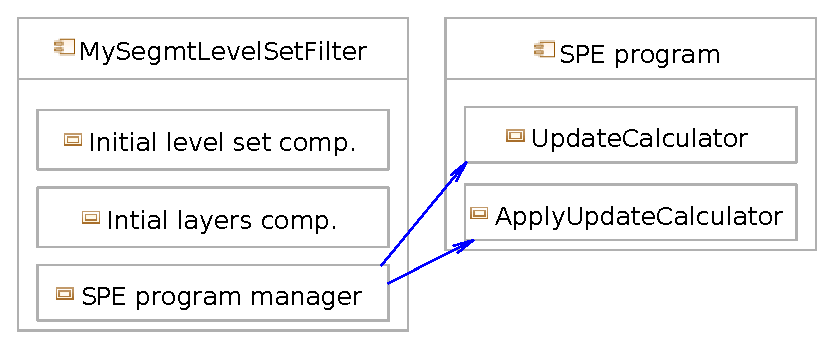
\includegraphics[width=0.9\textwidth]{data/newDesign}
    \caption[Diagram of new design components]{//TODO}
    \label{fg:newDesign}
\end{figure}

On the figure \ref{fg:newDesign} can be noticed that almost whole original ITK pipeline is offloaded to SPE.
Only initialization routines are left to PPE. This lead to create the SPE program manager that will manage computations on SPEs.
It is responsible for SPE thread initialization and run, and SPEs synchronization.

SPE part consists of two main parts.
UpdateCalculator, performing \emph{apply update calculation} and ApplyUpdateCalculator, performing \emph{apply update calculation}.
The UpdateCalculator contains //TODO. It traverse over \emph{layer0} and computes update values for points in that layer which are stored in \emph{update buffer}.
Then is the ApplyUpdateCalculator's turn.
It takes the update values from the \emph{update buffer} and performs all the steps from the sparse field algorithm \ref{alg:sparseFileld}.
This means:
\begin{enumerate}
\item STEP 2
\par
For every \emph{layer0} compute new level set value and perform test if it stays in the interval [-$\frac{1}{2}$,$\frac{1}{2}$].
If not, move the point into appropriate status list.
This is performed by \emph{UpdateActiveLayerValues} method.

\item STEP 3
\par
Is performed by subcomponent of ApplyUpdateCalculator, the LayerValuesPropagator.
This traverses over all layers, process their values and remove nodes eventually if they are no longer in a layer.
Step processed by \emph{PropagateAllLayerValues}.

\item STEP 4
\par
Traverse over status lists in innermost to outermost order and process their
nodes. If needed a node is moved to inward (outward) status list and
simultaneously appropriate layer. This is performed by \emph{ProcessStatusLists}
method.
\end{enumerate}

\subsection{Data flow}

In porting process is necessary to know the data flow i.e. find out what data are sent and where.
What data are there produced and especially the size of all the data.
This is because of decision where they will be stored.
Whether in SPE local store or in central memory.
For the first case their size has to be somehow limited because of limitation of local store.
For the second case communication via DMA will be necessary but the data size is not limited to small local store.

In my application following data flow:
\begin{enumerate}
\item UpdateCalculator
\par
Needs array which is as long as the layer0.
The size of a layer can be very big so it impossible to store it within SPE local store.
It has to reside in central memory and the layer's nodes has to be load into SPE local store while the list traversal.

\item \emph{UpdateActiveLayerValues}
\par
Process the array from UpdateCalculator so it has to load it from central memory.
It operates on layer0.
Some nodes are moved into status list and simultaneously \emph{UNLINKed} from layer0 list.
Layer resides in central memory so beside the loading nodes for traversing, some special operation has to be defined which perform the \emph{UNLINK} action.
\par
Status lists are temporary objects. They live only during one ApplyUpdateCalculator turn.
So they can reside within SPE's local store.
So no special operation communicating with central memory has to be defined.
But processing of the list0 has to be changed.
In original ITK code is \emph{UpdateActiveLayerValues} called on the whole layer0.
This one call can produce many of nodes that has to be put into a status list.
So iteration over layer0 has to be limited to produce limited amount of nodes to be put into status lists.
I defined the limit with constant MAX\_TURN\_LENGHT and call processing the limited segment of layer0 a 'turn'.
See figure \ref{fg:updateActiveLayerValues}.

\item \emph{ProcessStatusLists}
\par
Works on the status lists that reside within SPE's local store and are somehow limited in size (since the \emph{UpdateActiveLayerValues} run produce limited nodes into this status lists.
During processing this list nodes are linked into appropriate layer, this is another special operation communicating with central memory.
Lets call it \emph{PUSH}.
One status list processing empty the list so after \emph{ProcessStatusLists} run all status lists remains empty and are ready for next \emph{UpdateActiveLayerValues} turn.

\item \emph{ProcessStatusLists}
\par
This method traverse over all the layers and performs moving nodes among layers.
This means operations \emph{PUSH} and \emph{UNLINK}.
\end{enumerate}

\begin{figure}	//TODO
    \centering
    \includegraphics[width=0.9\textwidth]{data/updateActiveLayerValues}
    \caption[Diagram of new design components]{//TODO}
    \label{fg:updateActiveLayerValues}
\end{figure}

Status and actual level set values are stored within status and output images.
So for methods described above is necessary to load and store parts of that images.
Computation is performed on small neighbourhood of voxels 3x3x3.
So 27 voxels (resp. statuses) has to be transferred for one node processing.

There are some actions and operations defined above that need communication with central memory.
This is parts of program where cell PPE - SPE communication features take place.
Other SPE code need not to know if it is run on SPE or PPE (except case of vector intrinsics usage).

Because of separation of address spaces programming of SPE is very similar to client - server application design.
Roles depends on how the work is started.
In case PPU initiate the transfers the PPU is a client and SPE is a server (SPE receive some data for computation).
Another possibility that SPE grab the data from the central memory.
In this case SPE is client of central memory.
This case is prefered because the PPE is only one and would be able to manage all the SPU.

\subsection{Tools}
Some tools that performs data transfer between PPE and SPE was designed.
All these tools perform multibuffering to avoid waiting for data.

\begin{enumerate}
\item \emph{NeighbourhoodCell}
\par
Represent the part of an image ($3^3$ voxel matrix) needed for one node computation.
It uses transfer list that allow data handling in scatter-gather manner.
Neigbourhoods are grouped within PreloadedNeigborhoods container that manages which neigbourhood is being loaded, used in computation or saved (actually performs multibuffering)

\item \emph{RemoteArrayCell}
\par
Represent an array stored in main memory.
This tool is used for UpdateCalculator to save computed update values and in ApplyUpdateCalculator to retrieve the values which UpdateCalculator stored.
Its role is to perform DMA transfers not along each value save but on a buffer of that values.

\item \emph{LinkedChainIteratorCell}
\par
It traverse over a layer which is linked list data structure.
As soon as one item is retrieved, transfer of the next one is immediately started.
\end{enumerate}

\par
We decided to implement the \emph{PUSH} and \emph{UNLINK} operations through mailboxes.
Actual operation parameters are sent to PPE which performs the operation.
There are linked list manipulations performed within these operations and PPE can perform them directly (since it has direct access to central memory).
We believe that the linked list manipulations would be much more difficult and time consuming if performed by SPU because the indirect central memory access.

\begin{enumerate}
\item \emph{PUSH}
\par
Has to push a node into specified layer.
So only voxel coordinates and number of layer is send over mailbox to PPE that creates new node and puts it into the layer.

\item \emph{UNLINK}
\par
Operation has to unlink a node from a specified list.
Address of that node along the layer number are the parameters.
Address is transferred in 32 bits parts (because mailbox has 32 bit size) and is completed on the PPE side.
\end{enumerate}

Another support tool that is worth mention is \emph{ObjectStore} which is simple memory allocator templated with class that provides and size.
Provides two main methods, \emph{Borrow} and \emph{Return}.
It is used for allocation of status field nodes.
They resides in local store and thus should be allocated on stack.

Great advantage of the tools is also that the whole code uses only the tools (as instruments for central memory comunication).
So debuging transfer issues means debuging the tool.

\subsection{Work balancing}

The sparse field layers are central part that defines amount of work to be performed.
So it is necessary to balance their length among the SPE that process them.
This work is left to \emph{Work manager}.
Its goal is to ensure that all the layers are divided among SPE uniformly.

For this purpose the \emph{UNLINK} and \emph{PUSH} operations implemented using mailboxes fits well.
The idea behind is that actual operation on the linked list is delegated to the \emph{Work manager}.
It decides which layer segment (resp. SPE that the segment process) should the node append into.

\begin{figure}	//TODO obrazek
    \centering
    \includegraphics[width=0.9\textwidth]{data/updateActiveLayerValues}
    \caption[Diagram of new design components]{//TODO}
    \label{fg:updateActiveLayerValues}
\end{figure}

The whole process can be compared with company department where are several workers do actual work and one manager who distribute the work among the workers.

\section{Actual porting process}

\subsection{PC as simulator}
Because remote debugging program running on PS3 is quite time consuming (seconds for basic commands like step into) and because of small amount of memory (see \ref{ps3MemoryUsage}) we decided to left actual porting to the very end of process.
Features (and tools) that are needed for running on SPE were gradually added into the original code.
Some parts was rewritten (e.g. the \emph{UpdateActiveLayerValues} turn) to allow some data to live in SPE local store.
All the changes have not change the programs' output, so one can say that the all the programs in every step are equivalent.
All the debugging was performed on PC platform locally and thus quickly.
The Cell B.E. special features like DMA transfer was simulated by memcpy or the mailbox issues trough simple queue.

\par
This step was really time consuming due to fact that tools operates with stack memory.
Debuging such parts need extra care for what is where rewritten.
Since we are on stack some part of call stack would become corrupted and program becomes undefined.
The worst thing is that it can continue without crash or to crash on totaly different code that the error occured.
Errors of this type is always hard to track.
There is need of usage of some checking tools.
For us memcheck tool, part of Valgrind, proved to be useful to detect stack corruption.

\subsection{Moving to PPE}

\par
It seems that moving the code to PPE is easy and there could be no problem.
But we faced a problem that is worth to mention.
Because our code uses lot of third party libraries there is quite much paths to include folders.
It is neccessary to manage them well and not to mix alchitecture dependent ones.
We have mixed up include files of boost library when crosscompiling and experienced totally strange behavior.
We thaught that we can use includes for boost that come from repository for i686 architecture.
The code creashed on boost code that is debugged and stable.
Openning of a file have also crashed for unknown reason.
When program was compiled with includes from ppc(64) repository all problems disappeared.

\subsection{Tools porting}

\par
Next step was to port the tools for SPE.
In fact is to rewrite usage of memcpy that simulate the DMA trasfer to use real DMA transfer.

\par
Data that trasfered through DMA (DMAed) within Cell B.E. should meet size and align conditions (see \cite{programmersGuide}, Chapter 4).
Data that does not meet this condition will generate BUS error.
This condition forced that all data that are DMAed should be alocated onto aligned adresses (see objectStore.h or updateValsAllocator.h).

\par
Debuging within this step is performed already on Cell B.E. mashine.
We used both PS3 and systemsim.
Systemsim can detect which DMA transfer brakes align rules and thus cause the BUS error but it is really slow.
Instead using systemsim we have implement DMAGate (see DMAGate.h) that all DMA transfer go through and where are all the conditions checked.
Such central point for all DMA transfer is really important part of Cell B.E. program because it geathers all DMA stuff into one place making debuging much more easier.
